\subsection{Results for $x$ Offset}
%\label{subsec:longitude_no_abs_results}
%\vspace{10pt}

Figure~\ref{fig:var_long} represents the $p$-values for the Mann-Whitney $U$-test on actual and predicted values across $k$-fold validation datasets for the $x$ offset in the $k$-fold testing datasets using different RNN models, and forecasting times. Darker colors in grayscale represent a higher $p$-value in a range from $0$ to $1$. The values on the secondary diagonal are all equal to $1$ and black because models equal themselves.

\begin{figure}[!ht]
	\centering
	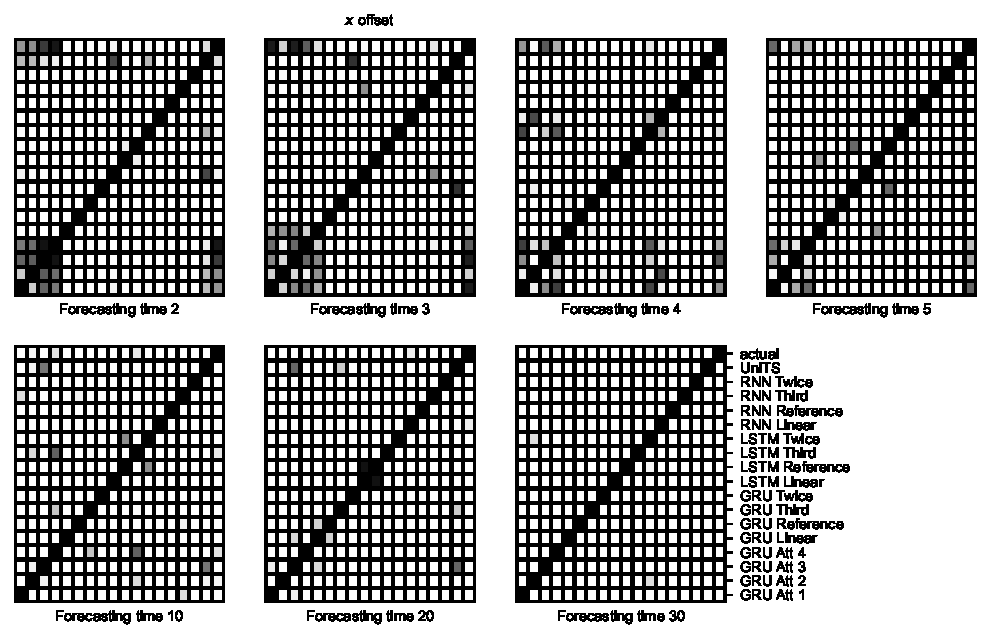
\includegraphics[width = 0.99 \linewidth]{var_long.pdf}
	\caption{The $p$-values for the Mann-Whitney $U$-test on actual and predicted values across $k$-fold validation datasets for the $x$ offset in the $k$-fold testing datasets using different RNN models, and forecasting times. Darker colors in grayscale represent a higher $p$-value in a range from $0$ to $1$. The values on the secondary diagonal are all equal to $1$ and black because models equal themselves.}
	\label{fig:var_long}
\end{figure}

The average $R^{2}$ (\%), with standard deviation in brackets, across $k$-fold validation datasets for the $x$ offset estimated on the $k$-fold testing datasets by different RNN models, and forecasting times is listed in Table~\ref{tab:best_longitude_no_abs_R2}.

\begin{table}[!ht]
	\centering
	\resizebox{\linewidth}{!}{
		\begin{tabular}{|c|c|c|c|c|c|c|c|}
			\hline
			Model & $2$ $s$ & $3$ $s$ & $4$ $s$ & $5$ $s$ & $10$ $s$ & $20$ $s$ & $30$ $s$ \\ \hline
			\multirow{2}{*}{GRU Att 1} & $95.29\%$ & $\mathbf{91.83\%}$ & $87.74\%$ & $84.62\%$ & $50.34\%$ & $14.63\%$ & $3.01\%$ \\
			 & ($0.92\%$) & \textbf{(}$\mathbf{1.53\%}$\textbf{)} & ($2.02\%$) & ($2.12\%$) & ($14.06\%$) & ($5.96\%$) & ($13.0\%$) \\ \hline
			\multirow{2}{*}{LSTM Third} & $\mathbf{96.88\%}$ & $89.96\%$ & $83.59\%$ & $76.3\%$ & $47.76\%$ & $-0.74\%$ & $-22.31\%$ \\
			 & \textbf{(}$\mathbf{1.13\%}$\textbf{)} & ($3.73\%$) & ($4.38\%$) & ($4.29\%$) & ($4.45\%$) & ($5.66\%$) & ($4.66\%$) \\ \hline
			\multirow{2}{*}{UniTS} & $93.99\%$ & $91.18\%$ & $\mathbf{88.19\%}$ & $\mathbf{85.09\%}$ & $\mathbf{69.54\%}$ & $\mathbf{42.6\%}$ & $\mathbf{23.39\%}$ \\
			 & ($0.83\%$) & ($1.05\%$) & \textbf{(}$\mathbf{1.32\%}$\textbf{)} & \textbf{(}$\mathbf{1.57\%}$\textbf{)} & \textbf{(}$\mathbf{2.54\%}$\textbf{)} & \textbf{(}$\mathbf{3.68\%}$\textbf{)} & \textbf{(}$\mathbf{4.0\%}$\textbf{)} \\ \hline
		\end{tabular}
	}
	\caption{The average $R^{2}$ (\%), with standard deviation in brackets, across $k$-fold validation datasets for the $x$ offset estimated on the $k$-fold testing datasets by different RNN models, and forecasting times.}
	\label{tab:best_longitude_no_abs_R2}
\end{table}

The GRU Att 1 model achieved the highest $R^{2}$ (\%) for $x$ offset, and a forecasting time of $3$ $s$ with an average value and standard deviation (in brackets) that equals $91.83$\% ($1.53$\%).

The GRU Att 1 model does not make statistically significantly different predictions than the GRU Att 2, GRU Att 3, GRU Att 4, GRU Linear, LSTM Linear, RNN Third, and actual value models for $x$ offset using a forecasting time of $3$ $s$, with $p$-values equaling $0.175$, $0.968$, $0.571$, $0.304$, $0.004$, $0.023$, and $0.9$.

\markertable{tab:\label{tab:longitude:no:abs:p:3}}

The LSTM Third model achieved the highest $R^{2}$ (\%) for $x$ offset, and a forecasting time of $2$ $s$ with an average value and standard deviation (in brackets) that equals $96.88$\% ($1.13$\%).

The LSTM Third model does not make statistically significantly different predictions than the LSTM Reference model for $x$ offset using a forecasting time of $2$ $s$, with a $p$-value equaling $0.063$.

\markertable{tab:\label{tab:longitude:no:abs:p:2}}

The UniTS model achieved the highest $R^{2}$ (\%) for $x$ offset, and a forecasting time of $4$, $5$, $10$, $20$, and $30$ $s$ with average values and standard deviation (in brackets) that equal $88.19$\% ($1.32$\%), $85.09$\% ($1.57$\%), $69.54$\% ($2.54$\%), $42.6$\% ($3.68$\%), and $23.39$\% ($4.0$\%) respectively.

The UniTS model does not make statistically significantly different predictions than the GRU Att 3, and actual value models for $x$ offset using a forecasting time of $4$ $s$, with $p$-values equaling $0.002$, and $0.003$.

\markertable{tab:\label{tab:longitude:no:abs:p:4}}

The UniTS model does not make statistically significantly different predictions than the GRU Att 3, GRU Twice, LSTM Third, and actual value models for $x$ offset using a forecasting time of $5$ $s$, with $p$-values equaling $0.016$, $0.003$, $0.063$, and $0.005$.

\markertable{tab:\label{tab:longitude:no:abs:p:5}}

The UniTS model does not make statistically significantly different predictions than the GRU Att 2, GRU Att 3, LSTM Reference, LSTM Twice, and actual value models for $x$ offset using a forecasting time of $10$ $s$, with $p$-values equaling $0.046$, $0.54$, $0.007$, $0.001$, and $0.0$.

\markertable{tab:\label{tab:longitude:no:abs:p:10}}

The UniTS model does not make statistically significantly different predictions than the GRU Att 3, and GRU Third models for $x$ offset using a forecasting time of $20$ $s$, with $p$-values equaling $0.976$, and $0.204$.

\markertable{tab:\label{tab:longitude:no:abs:p:20}}

The average MAE in $\degree$ ($\times 10^{-5}$), with standard deviation in brackets, across $k$-fold validation datasets for the $x$ offset estimated on the $k$-fold testing datasets by different RNN models, and forecasting times is listed in Table~\ref{tab:best_longitude_no_abs_MAE}.

\begin{table}[!ht]
	\centering
	\resizebox{\linewidth}{!}{
		\begin{tabular}{|c|c|c|c|c|c|c|c|}
			\hline
			Model & $2$ $s$ & $3$ $s$ & $4$ $s$ & $5$ $s$ & $10$ $s$ & $20$ $s$ & $30$ $s$ \\ \hline
			\multirow{2}{*}{GRU Att 1} & $\mathbf{6.81}$ & $\mathbf{9.13}$ & $\mathbf{11.39}$ & $\mathbf{12.77}$ & $25.31$ & $37.95$ & $42.58$ \\
			 & \textbf{(}$\mathbf{0.85}$\textbf{)} & \textbf{(}$\mathbf{1.09}$\textbf{)} & \textbf{(}$\mathbf{1.48}$\textbf{)} & \textbf{(}$\mathbf{1.41}$\textbf{)} & ($5.26$) & ($3.28$) & ($3.71$) \\ \hline
			\multirow{2}{*}{GRU Att 2} & $7.15$ & $9.67$ & $11.58$ & $13.14$ & $\mathbf{20.61}$ & $31.95$ & $40.63$ \\
			 & ($0.86$) & ($1.3$) & ($1.44$) & ($2.01$) & \textbf{(}$\mathbf{2.81}$\textbf{)} & ($3.97$) & ($4.81$) \\ \hline
			\multirow{2}{*}{UniTS} & $9.01$ & $11.04$ & $12.85$ & $14.49$ & $21.05$ & $\mathbf{29.73}$ & $\mathbf{35.17}$ \\
			 & ($0.96$) & ($1.19$) & ($1.38$) & ($1.55$) & ($2.2$) & \textbf{(}$\mathbf{3.04}$\textbf{)} & \textbf{(}$\mathbf{3.37}$\textbf{)} \\ \hline
		\end{tabular}
	}
	\caption{The average MAE in $\degree$ ($\times 10^{-5}$), with standard deviation in brackets, across $k$-fold validation datasets for the $x$ offset estimated on the $k$-fold testing datasets by different RNN models, and forecasting times.}
	\label{tab:best_longitude_no_abs_MAE}
\end{table}

The GRU Att 1 model achieved the lowest MAE for $x$ offset, and a forecasting time of $2$, $3$, $4$, and $5$ $s$ with average values and standard deviation (in brackets) that equal $6.81 \times 10^{-5}$ $\degree$ ($0.85 \times 10^{-5}$ $\degree$), $9.13 \times 10^{-5}$ $\degree$ ($1.09 \times 10^{-5}$ $\degree$), $11.39 \times 10^{-5}$ $\degree$ ($1.48 \times 10^{-5}$ $\degree$), and $12.77 \times 10^{-5}$ $\degree$ ($1.41 \times 10^{-5}$ $\degree$) respectively.

The GRU Att 1 model does not make statistically significantly different predictions than the GRU Att 2, GRU Att 3, GRU Att 4, LSTM Linear, LSTM Twice, UniTS, and actual value models for $x$ offset using a forecasting time of $2$ $s$, with $p$-values equaling $0.954$, $0.611$, $0.524$, $0.052$, $0.02$, $0.265$, and $0.412$.

The GRU Att 1 model does not make statistically significantly different predictions than the GRU Att 2, GRU Att 3, GRU Att 4, GRU Linear, LSTM Linear, RNN Third, and actual value models for $x$ offset using a forecasting time of $3$ $s$, with $p$-values equaling $0.175$, $0.968$, $0.571$, $0.304$, $0.004$, $0.023$, and $0.9$.

The GRU Att 1 model does not make statistically significantly different predictions than the GRU Att 2, GRU Att 3, GRU Att 4, LSTM Twice, RNN Linear, and actual value models for $x$ offset using a forecasting time of $4$ $s$, with $p$-values equaling $0.063$, $0.45$, $0.756$, $0.728$, $0.054$, and $0.417$.

The GRU Att 1 model does not make statistically significantly different predictions than the GRU Att 2, GRU Att 3, GRU Att 4, and actual value models for $x$ offset using a forecasting time of $5$ $s$, with $p$-values equaling $0.031$, $0.332$, $0.574$, and $0.595$.

The GRU Att 2 model achieved the lowest MAE for $x$ offset, and a forecasting time of $10$ $s$ with an average value and standard deviation (in brackets) that equals $20.61 \times 10^{-5}$ $\degree$ ($2.81 \times 10^{-5}$ $\degree$).

The GRU Att 2 model does not make statistically significantly different predictions than the GRU Att 3, LSTM Third, UniTS, and actual value models for $x$ offset using a forecasting time of $10$ $s$, with $p$-values equaling $0.055$, $0.145$, $0.046$, and $0.037$.

The UniTS model achieved the lowest MAE for $x$ offset, and a forecasting time of $20$, and $30$ $s$ with average values and standard deviation (in brackets) that equal $29.73 \times 10^{-5}$ $\degree$ ($3.04 \times 10^{-5}$ $\degree$), and $35.17 \times 10^{-5}$ $\degree$ ($3.37 \times 10^{-5}$ $\degree$) respectively.

The UniTS model does not make statistically significantly different predictions than the GRU Att 3, and GRU Third models for $x$ offset using a forecasting time of $20$ $s$, with $p$-values equaling $0.976$, and $0.204$.

